\subsubsection{Strategy}

Il pattern Strategy è utilizzato quando occorre definire una famiglia di
algoritmi e renderli intercambiabili, permettendo loro di variare
indipendentemente dal client.

Oggetti Strategy possono essere utilizzati per fornire diverse implementazioni
di uno stesso algoritmo o comportamento, e il client può scegliere il più
appropriato in base ai diversi \frgnword{trade-off} di tempo e spazio.

\begin{figure}[h!]
  \centering
  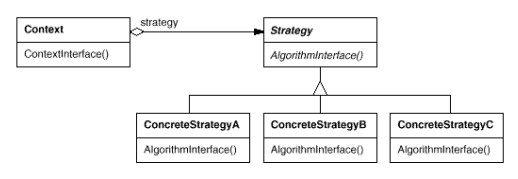
\includegraphics[scale=0.55]{imgs/strategy.jpg}
  \caption{Diagramma delle classi del pattern Strategy}
\end{figure}

La classe base comune a tutti gli oggetti Strategy permette di fattorizzare
eventuale logica in comune.

\paragraph{Vantaggi}

La presenza di più comportamenti è modellabile con l'ereditarietà, dove ogni
sottoclasse implementa un algoritmo differente per la stessa operazione. In
questo modo, però, la sottoclasse è legata staticamente all'algoritmo, e può
generare una moltitudine di sottoclasssi che differiscono tra loro solamente per
il comportamento.

Il pattern Strategy permette di variare algoritmi diversi dinamicamente, e
indipendentemente dal contesto di utilizzo, eliminando il bisogno di
\frgnword{statement} condizionali per selezionare il comportamento più
appropriato.

\paragraph{Svantaggi}

Il client deve comprendere la differenza tra i diversi Strategy, per selezionare
quello più appropriato. Pertanto, tale pattern va utilizzato solamente se la
variazione di comportamento è rilevante per il codice client.

Un'altro svantaggio riguarda l'incremento del numero di oggetti presenti a
runtime conseguente dall'uso del pattern. Tale numero può essere ridotto
implementando gli Strategy come oggetti \frgnword{stateless}, permettendo a più
client di condividere istanze.

\paragraph{Implementazione}

Tutte le classi rappresentanti uno Strategy devono aderire ad un'interfaccia
comune, che deve essere opportunamente progettata. Tale interfaccia deve
costituire un efficace punto di accesso dallo Strategy al contesto di utilizzo,
e viceversa.

Un possibile approccio consiste nel passare i dati necessari allo Strategy per
parametro. Questo permette un basso accoppiamento, ma la presenza di troppi
parametri potrebbe fare in modo che alcuni Strategy concreti usino solo
parte di essi, facendo istanziare al client oggetti che non verranno utilizzati.

Un'altra possibile implementazione vede il client passare se stesso come
parametro allo Strategy, o lo Strategy avere un riferimento al suo client.
Questo elimina il bisogno di passare parametri, e il possibile spreco di essi,
ma richiede che il client definisca un'interfaccia più elaborata per l'accesso
ai suoi dati, aumentando l'accoppiamento tra i due elementi.
